\documentclass[a4paper, 12pt]{article}

\usepackage[czech]{babel}
\usepackage{graphicx}
\usepackage[utf8]{inputenc}
\usepackage{listings}
\usepackage{url}
\usepackage[usenames]{xcolor}
% \usepackage{a4wide}

\DeclareUrlCommand\url{\def\UrlLeft{<}\def\UrlRight{>} \urlstyle{tt}}

\lstset{language=Java}

\begin{document}
\begin{titlepage}

\includegraphics{fav_cmyk.pdf}
\vfill
\begin{center}
{\huge Umělá inteligence a rozpoznávání}\\[3ex]
{\Large Expertní genealogický systém}
\end{center}
\vfill
\begin{tabbing}
Vypracoval: \hspace{1ex}\=Zdeněk Janeček\kill
Vypracoval: \>Zdeněk \textsc{Janeček}\\[1ex]
Datum:\> \today
\end{tabbing}
\end{titlepage}

\section{Zadání}
Vytvořte genealogický expertní systém. Vstupem bude informace databáze
základních informací o osobě [id, jméno, matka, otec, pohlaví, partner].
Program bude umět odpovídat na otázky: Kdo je můj pokrevní příbuzný?
Kolik má moje prateta sestřenic? Jaký je vtah mezi Petrem a Pavlem?\ldots
a další podobné.

\section{Analýza}
% TODO: alternativní řešení
Rodinný strom je z hlediska grafové teorie n-ární strom, protože mám dva
rodiče a neomezeně mnoho dětí. Pokud zanedbám manželství a postavím
strom jen ze vztahů rodič--potomek, bude požadovaná acykličnost grafu
zachována.
Manželství není stálé a stačí si ho tedy pouze zaznamenat.
Společné děti manželů, také nejsou jisté, tudíž je praktičtější ukládat
si potomky u každého rodiče zvlášť.

Jak tedy dobře reprezentovat tento strom aby se dobře prohledával?
První co mě napadne je, že každý uzel bude jeden objekt a bude mít
odkazy na své potomky a rodiče. Na vyhodnocování zvolím algoritmy
jako na každý graf. Mohl jsem ale jít cestou znalostní báze. Ta by
shromažďovala všechna známá i nově nalezená fakta. Tento přístup
by byl určitě flexibilnější, ale na něj by byl vhodnější jazyk \emph{Prolog}.
Měl jsem nápad že by byl vhodný také konečný automat. Nakonec něco
na ten způsob jsem také trochu použil. Nemělo cenu zavádět gramatiku.

Abych mohl ukládat rodinný strom, je třeba stanovit jeho kořen. Mám tedy
dvě varianty. Kořenem bude jeden společný potomek, a nebo společná
matka. Zvolil jsem jako kořenový uzel supermatku, která dostala id 0.

Pro ukládání dat o rodině jsem vytvořil jednoduchý formát souboru.
Na obrázku \ref{fig:familyk} vidíte následující položky:

\begin{enumerate}
\setcounter{enumi}{-1}
\item ID
\item Jméno
\item (červeně) id natky
\item (azurová) id otce
\item (zelené) true -- muž, false -- žena
\item (modře) partner, nemá partnera pak \emph{nil}
\end{enumerate}

Když víme počet položek z prvního řádku, algoritmus je pak jednoduchý:
\begin{enumerate}
\item načti atributy
\item když neexistuje osoba, vytvoř její základ
\item přidej se jako dítě rodiče a nastav partnera. Pokud ještě neexistuji, vytvoř je
\item aktualizuj informace o sobě
\item opakuj krok 1 pro další osobu
\end{enumerate}
\begin{figure}
\centerline{\begin{minipage}{0.65\textwidth}
{
\Large\sffamily
9\\[3pt]
[1, Kocourek Petr, \textcolor{red}{4}, \textcolor{cyan}{3}, \textcolor{green}{true}, \textcolor{blue}{nil}]\\[3pt]
[4, Kocourková Ivana, \textcolor{red}{8}, \textcolor{cyan}{9}, \textcolor{green}{false}, \textcolor{blue}{3}]
}
\end{minipage}}
\caption{Formát souboru s rodinnými daty.}
\label{fig:familyk}
\end{figure}

Jakmile máme vytvořený strom, lze na něm dělat standardní
prohledávání a sledovat, zda jsme dostáli požadovaného výsledku.

\section{Vyhodnocování}
Při zápisu výstupu byly použity escape sekvence,
které umožňují mazat kusy obrazovky a tím dosáhnout určité
interaktivity. Budou stačit dva způsoby vstupu a to pro \emph{id osoby} a
požadovaný vztah. V hlavičce programu se bude vypisovat formulovaná
otázka. Více v sekci \ref{sec:int} na straně \pageref{sec:int}.

Uvnitř programu zastupuje třída \texttt{NTree} rodinný strom. Tato třída je
konstruována s parametrem souboru s rodinnými daty. Při vytvoření se soubor
načte a vytvoří pole instancí třídy \texttt{Node}. Nyní máme k dispozici
například metodu \texttt{void printTree()}, která vytiskne strom na
obrazovku. Každý \texttt{Node} představuje jednu osobu. Procházení stromu
je pak rychlé, protože můžu využít jak tabulku, tak odkaz na sousední uzel.
Veškeré dotazy na uzel se pak provádí v čase $\mathcal{O}(1)$.

Další část je práce s expertními daty. Bylo třeba navrhnout jak
reprezentovat rodinný vztah. Využil jsem predikátové logiky,
která je dostatečně univerzální pro práci s množinou prvků.
Definoval jsem například:

\begin{equation}
P(x,a) \wedge P(a,b) \wedge C(b,c) \wedge N(c,a) \rightarrow \mbox{\emph{c} je sourozenec rodičů}
\label{eq:rule}
\end{equation}

Vystačil jsem si se třemi funkcemi říkající:
\begin{description}
\item[P(a,b)] rodiče termu \emph{a} jsou \emph{b}.
\item[C(a,b)] děti termu \emph{a} jsou \emph{b}.
\item[N(a,b)] term \emph{a} neobsahuje prvky z \emph{b}.
\end{description}

Soubor jsem navrhl podobně. Stačilo se zbavit závorek a konjunkcí,
které budou platit vždy a není tedy nutné je ukládat. Soubor má formát
podle obrázku \ref{fig:expert}. První řádek je opět počet položek
v tomto souboru. Každé pravidlo má dva řádky. První z nich obsahuje
popis vztahu a na dalším je samotné pravidlo.

\begin{figure}
\centerline{\begin{minipage}{0.65\textwidth}
{
\Large\sffamily
2\\[3pt]
[3, \textcolor{magenta}{prarodič}, \textcolor{cyan}{dědeček}, \textcolor{green}{babička}]\\[3pt]
PxaPab\\[3pt]
[4, \textcolor{magenta}{sourozenec rodičů}, \textcolor{cyan}{strýc}, \textcolor{green}{teta}]\\[3pt]
PxaPabCbcNca
}
\end{minipage}}
\caption{Formát souboru s expertními daty.}
\label{fig:expert}
\end{figure}

Nyní bude následovat popis vnitřních částí třídy \texttt{Expert}.
Tyto metody volá třída \texttt{Starter}, která zobrazuje výsledky otázek.

\subsection{Využité nástroje}
Užitečná je metoda na nalezení id vztahu, pokud mám zjednodušené
pravidlo bez termů jako například PCC místo PabCbcCcx.

\begin{verbatim}
public int getRealationId(String rule) {
    for (int i = 0; i < relations.length; i++) {
        if (compareRel(relations[i].rule, rule)) {
            return i;
        }
    }
    return -1;
}
\end{verbatim}

\subsection{Metoda findPerson}
Pokud potřebuji odpovědět na otázky typu:

\begin{quote}
V jakém vztahu jsou Petr a Ivana?
\end{quote}

\begin{verbatim}
/**
 * Searches for some person and returns their relation.
 * 
 * @param from Person to search from.
 * @param target Person to search for.
 * @return result of search
 */
public String findPerson(Node from, Node target) {}
\end{verbatim}

Prohledáváním do šířky od uzlu \texttt{from} přidávám každému
nově nalezenému uzlu záznam o jeho cestě. Ukládám si pole
\texttt{paths}, kde jsou řetězce ve stylu PCC. Do fronty \texttt{q}
přidávám jak jeho děti, tak rodiče.

Naleznu-li požadovanou osobu, najdu jakému odpovídá vztahu
a vrátím řetězec podle vzoru:

\begin{quote}
Nalezen  [jmeno] ve vztahu [vztah]
\end{quote}

\subsection{Metoda findPersons}
Pokud potřebuji odpovědět na otázky typu:

\begin{quote}
Kdo všechno jsou bratranci zadané osoby?
\end{quote}

\begin{verbatim}
/**
 * Finds all persons in specified relation.
 * 
 * @param from Person to search from.
 * @param rel wanted relation
 * @param male is male or female
 * @return LinkedList of person instances
 */
public Collection<Node> findPersons(Node from,
    int rel, boolean male) {}
\end{verbatim}

Prohledáváním do šířky od uzlu \texttt{from} přidávám každému
nově nalezenému uzlu záznam o jeho cestě. Ukládám si pole
\texttt{paths}, kde jsou řetězce ve stylu PCC. Do fronty \texttt{q}
přidávám jak jeho děti, tak rodiče.

Rezoluce, zda \texttt{v} je hledaná osoba, vypadá následovně:

\begin{verbatim}
if (v.isMale()==male && compareRel(rule, paths[v.getId()])) {
    result.add(v);
}
\end{verbatim}

Vzniklý seznam \texttt{result} vracím jako návratová hodnota.

\subsection{Metoda testRelation}
Pokud potřebuji odpovědět na otázky:

\begin{quote}
Jsou tyto osoby v daném vztahu?
\end{quote}

\begin{verbatim}
/**
 * @param from From which person is done an comparison.
 * @param target To which person is done an comparison.
 * @param rel relation id we want to test
 * @param male true if I look for male, false if it is female
 * 
 * @return true if it founds the person and the false in
 *         the other case
 */
public boolean testRelation(Node from, Node target,
    int rel, boolean male) {}
\end{verbatim}

V tomto případě se nejedná o slepé prohledávání, ale přesně podle
daného pravidla. Vedu si evidenci o každém symbolu, který
jsem našel. Mohu se tedy pak vracet k nějaké starší množině lidí.
Při provádění pravidla využívá funkcí jak byly definovány ve vzoru \ref{eq:rule}.
První znak je zdroj a druhý je cíl. Na konci se musí hledaná osoba nalézat
v poslední zpracované množině.

\section{Metoda bloodLine}
Pokud potřebuji odpovědět na otázku:

\begin{quote}
Kdo jsou pokrevní příbuzní dané osoby?
\end{quote}

\begin{verbatim}
/**
 * Get your blood line. They are all parents of parents
 * and so on.
 * @param from Person to search from.
 * @param deep how deep you want to search
 * @return all persons that are my ascendants
 */
public Collection<Node> bloodline(Node from, int deep) {}
\end{verbatim}

S použitím dvou stavových proměnných a jedním čítačem
je omezeno prohledávání do šířky. Prohledávání se líší od
předchozích jen tím, že přidávám do fronty jen rodiče.

\section{Interakce s uživatelem}\label{sec:int}
O uživatelské prostředí se stará třída \texttt{Starter}.
Je tedy nutné používat terminál,
který je podporuje ANSI ecape kódy\footnote{\url{http://en.wikipedia.org/wiki/ANSI_escape_codes}}.

\begin{figure}
\centering
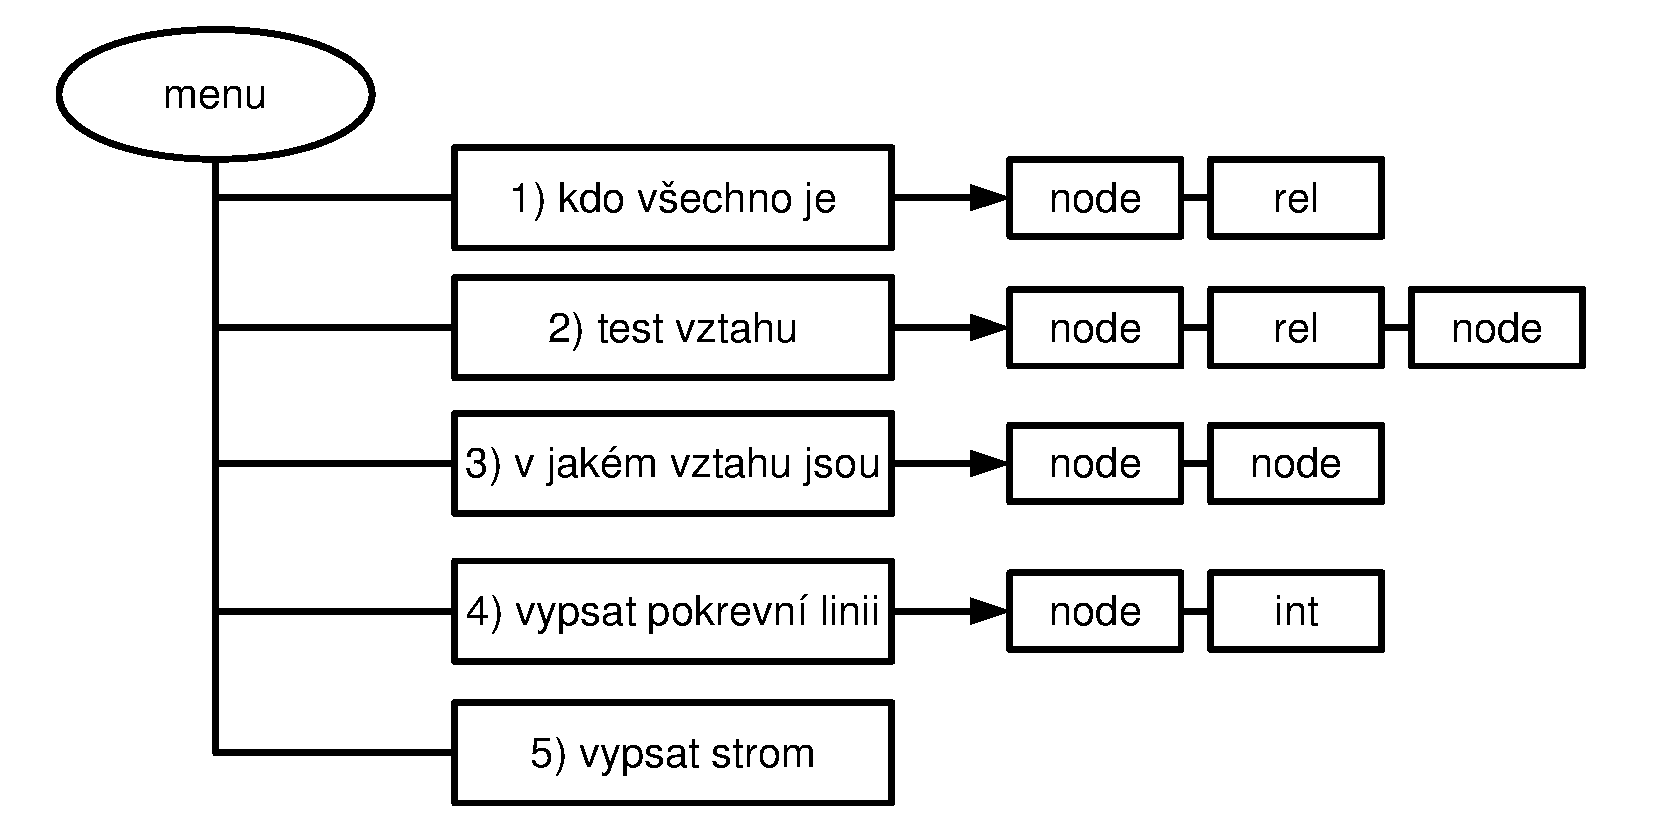
\includegraphics[width=\textwidth]{menu}
\caption{Typy vstupních dat.}
\label{fig:input}
\end{figure}

Vytvořil jsem obrázek \ref{fig:input}, na kterím lze snadno vyčíst
jaký typ dat je očekáván pro jednotlivé otázky. Blok \textsf{node}
otázku na osobu, \textsf{rel} otázku na vztah (např. bratranec)
a poslední \textsf{int} načítání celočíselné hodnoty.

Pro účely testování je možné použít soubor \textsf{familyData},
ve kterém je uložen rodokmen z obrázku \ref{fig:family}.

\begin{figure}
\centering
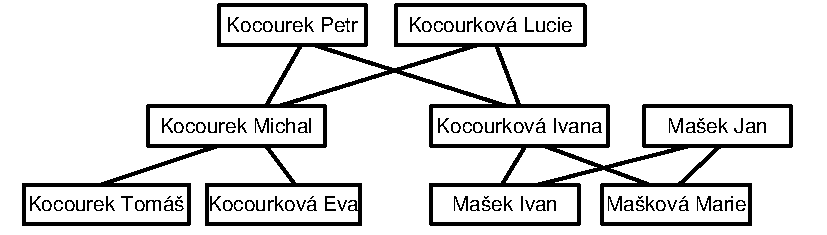
\includegraphics[width=\textwidth]{testData}
\caption{Vzorová rodinná data.}
\label{fig:family}
\end{figure}

\section{Spouštění a obsluha}
K dispozici je popisový soubor \textsf{build.xml}. Pro překlad a spuštění
stačí spustit:
\begin{verbatim}
$ ant
$ java -cp bin/ kiv.janecekz.Starter
\end{verbatim}

Pokud po aplikace požaduje nějaký vstup, poznáte to podle
znaků $>>$. Vstupem může být číslo, nebo řetězec. To je
rozepsáno na obrázku \ref{fig:input}.

\section{Shrnutí}
Při psaní jsem několikrát lehce změnil návrh. V počátku jsem o expertním
systému nevěděl vůbec nic, takže jsem použil již ověřené postupy.
Aplikace byla napsána pomocí Eclipse IDE a dokumentace vysázena systémem
\LaTeX{}. Projekt má svůj Git repositář na adrese
\url{https://github.com/qwertzdenek/genealogy}.

\end{document}
